\newcommand{\class}[1]{\texttt{#1}}
\newcommand{\method}[1]{\texttt{#1}}
\newcommand{\attr}[1]{\textit{#1}}

Im Folgenden werden einige Designentscheidungen des Projekts beschrieben.
Dazu werden zuerst die entworfenen Klassen mit deren Attributen und Methoden beschriebenen.
Danach werden einige Verhaltensaspekte mit Sequenzdiagramm veranschaulicht.

\subsection{Struktur}
Diagramm \ref{fig:class_diagramm} zeigt alle Klassen des Projekts mit deren Beziehungen, Attributen und Methoden.


\begin{figure}[htbp]
	\centering
	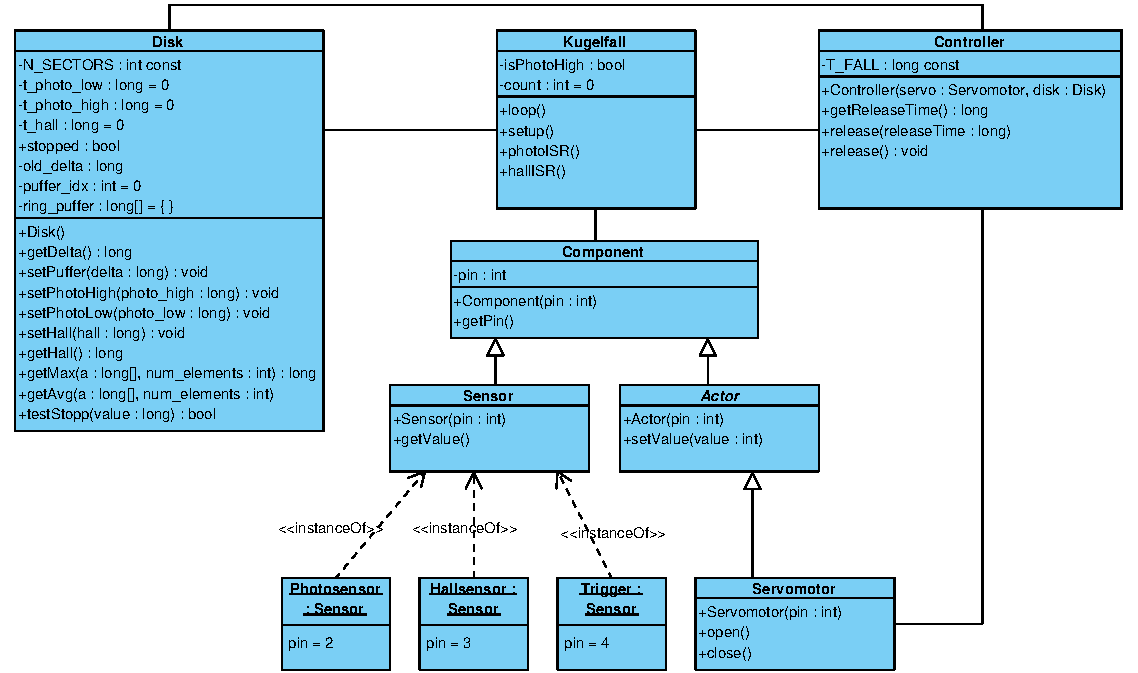
\includegraphics[width=\textwidth]{abb/class_cropped}
	\caption{Klassen mit deren Beziehungen, Methoden und Attributen}
	\label{fig:class_diagramm}
\end{figure}

\paragraph{\class{Kugelfall}}
ist die zentrale Klasse, da sie die Arduino-Methoden \method{setup()} und \method{loop()} enthält.
Sie steht in Beziehung zur allen anderen Klassen.
Innerhalb der \method{setup()}-Methode initialisiert sie die anderen Projekt-Klassen mit den entsprechenden Parametern (siehe Diagramm \ref{fig:setup_diagram}).
Ebenso werden die Interrupts zum Photosensor und Hallsensor mit den Methoden \method{photoISR()} bzw. \method{hallISR()} initialisiert (siehe Diagramm \ref{fig:photoISR} und \ref{fig:hallISR}).
Innerhalb der \method{loop()}-Methode wird auf Triggerdruck des Nutzers gewartet und ggf. der Mechanismus zur Berechnung der Fallzeit und das Loslassen aufgerufen (siehe Diagramm \ref{fig:loop_diagram}).

\paragraph{\class{Component}} entspricht einer Hardware-Komponente, auf welche mittels Arduino zugegriffen werden kann.
Es besitzt als einziges Attribut den \attr{pin} der Arduino-Komponente, welcher im Konstruktor initialisiert wird und mittels der Funktion \method{getPin()} abgerufen werden kann.

\paragraph{\class{Sensor}} entspricht einem Hardware-Sensor und ist eine Spezialisierung der Klasse \class{Component}. 
Es initialisiert die Instanz mit dem Pin-Modus \texttt{INPUT\_PULLUP} und dem übergebenen Pin.
Die Methode \method{getValue()} liest zur Aufrufzeit den entsprechenden Wert aus.
Dabei gibt es bei diesem Projekt insgesamt die drei Sensor-Exemplare \textit{Photosensor}, \textit{Hallsensor} und \textit{Trigger}, die jeweils mit den entsprechenden Pins initialisiert wurden. 

\paragraph{\class{Actor}} entspricht einem Hardware-Aktor und ist eine Spezialisierung der Klasse \class{Component}.
Es initialisiert die Instanz mit dem Pin-Modus \texttt{OUTPUT} und dem übergebenen Pin.
Die Methode \method{setValue()} schreibt den übergebenen Wert zum Aktor.

\paragraph{\class{Servomotor}} entspricht einem Hardware-Servomotor und ist eine Spezialisierung der Klasse \class{Actor}.
Es initialisiert im Konstruktur den Servomotor mit dem entsprechenden Pin.
Die Methoden \method{open()} und \method{close()} dienen zum Öffnen und Schließen des Servomotors und damit der Fallvorrichtung.

\paragraph{\class{Disk}} entspricht der Scheibe des Kugelfallaufbaus.
Neben festen Spezifikationen wie die Anzahl der Sektoren hat es auch die Attribute zum Festhalten der letzten Zeiten für Photosensor  (\method{setPhotoLow()}, \method{setPhotoHigh()}) und Hallsensor (\method{setHall()}). 
Zur Speicherung der Unterschiede der Zeitpunkte für steigende und fallende Flanke des Photosensor (Delta-Werte) nutzt es einen Ringpuffer, sodass die 24 zuletzt ermittelten Delta-Werte gespeichert werden (siehe Diagramm \ref{fig:photoISR}).
Zur Rückgabe eines Delta-Wertes (\method{getDelta()}) aus dem Ringpuffer wird die Funktion \method{getMax()} (bzw. \method{getAvg()}) verwendet.
So können Fehler aufgrund von Messungenauigkeiten kompensiert werden.

\paragraph{\class{Controller}} dient zur Berechnung der Fallzeit und dem Loslassen der Kugeln.
So dient die Methode \method{waitForRelease()} zur der Berechnung Loslasszeit, dem Warten auf die korrekt Fallzeit und dann dem Loslassen (siehe Diagramm \ref{fig:loop_diagram}).
Zur Berechnung der Fallzeit dient die Methode \method{getReleaseTime()}, welche dabei die feste Fallzeit der Kugel \attr{T\_FALL}, einen dynamischen Delay (\method{getDynamicDelay()} und die Delta-Werte des Photosensors der Klasse \class{Disk} benutzt (näheres siehe Abschnitt \ref{ssec:nutzung}).
Für das Fallenlassen mit der Methode \method{release()} nutzt es die Klasse \class{Servomotor}.

\subsection{Verhalten}
Im Folgenden werden einige Verhaltensaspekte beschrieben.

Diagramm \ref{fig:setup_diagram} zeigt die Initialisierung der Anwendung mittels der Methode \method{setup} der Klasse \class{Kugelfall}.
\begin{figure}[htbp]
	\centering
	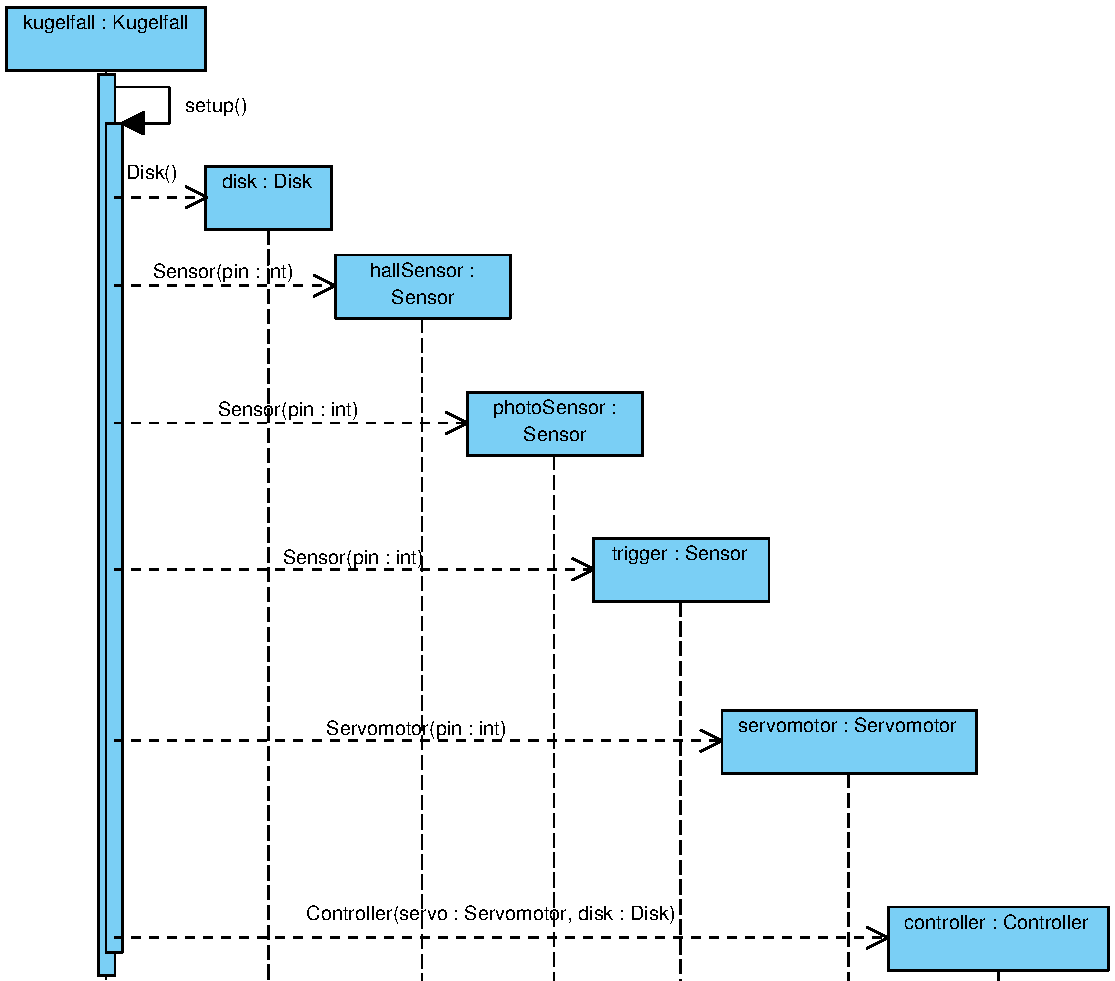
\includegraphics[width=\linewidth]{abb/setup_cropped}
	\caption{Ablauf bei der Methode \method{setup} von Klasse \class{Kugelfall}}
	\label{fig:setup_diagram}
\end{figure}
Dabei werden nacheinander die einzelnen Klassen instantiiert. 
Bei den Sensoren müssen die spezifischen Pins angegeben werden.
Bei der Initialisierung des \class{Controller} werden die Instanzen der Klassen \class{Servomotor} und \class{Disk} mit übergeben.

Diagramm \ref{fig:loop_diagram} zeigt auf sehr übersichtliche Art den Ablauf in der Dauerschleife in der Methode \method{loop()}.
\begin{figure}[htbp]
	\centering
	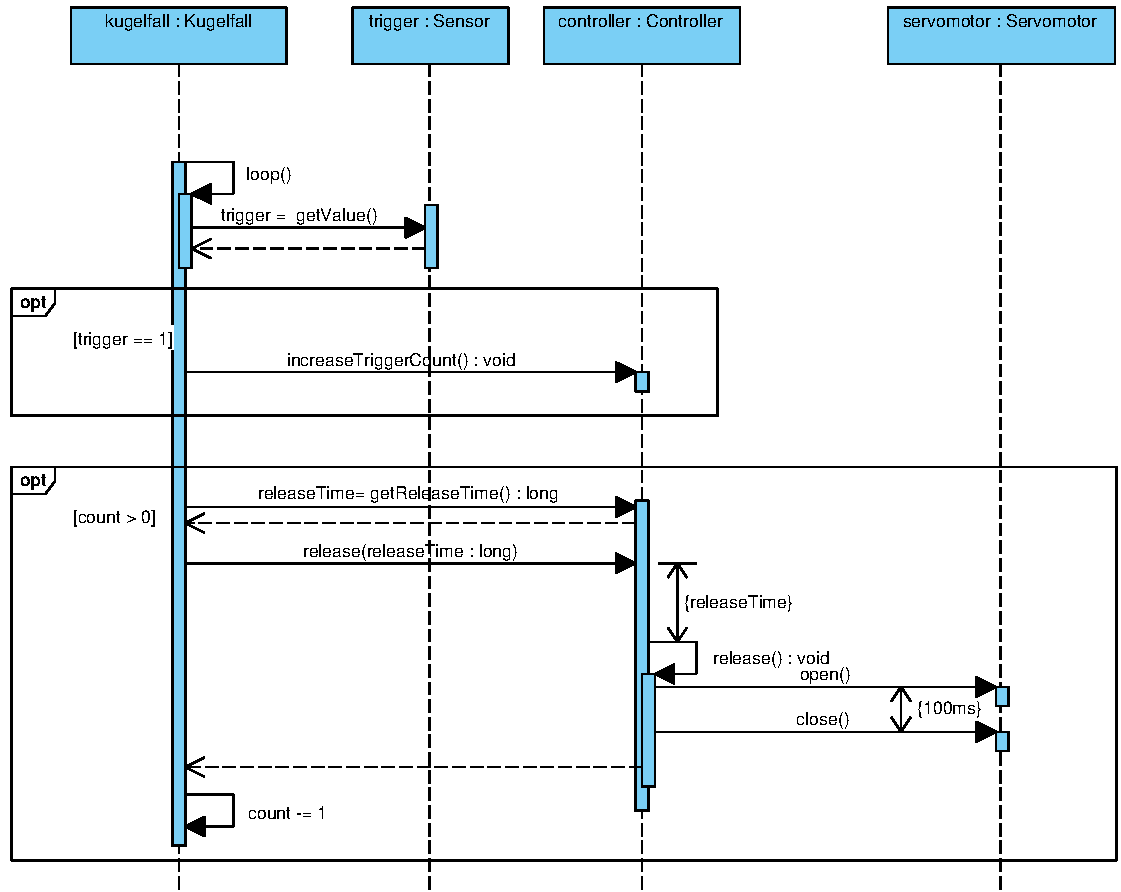
\includegraphics[width=\textwidth]{abb/loop_cropped}
	\caption{Ablauf bei der Methode \method{loop} von Klasse \class{Kugelfall}}
	\label{fig:loop_diagram}
\end{figure}
So wird zuerst der Triggerwert ausgelesen und damit geguckt, ob er vom Nutzer gedrückt wurde.
Ist das der Fall wird der Triggerzähler um eins erhöht.
Ist der Zähler derzeit größer null wird die Berechnung der Fallzeit und das Loslassen der Kugel mit der Methode \method{waitForRelease()} gestartet.
Dabei wird in der Dauerschleife zuerst mit der Methode \method{isSteady()} der Klasse \class{Disk} geprüft, ob sich die Scheibe derzeit stabil dreht.
Nur im Falle einer stabil drehenden Scheibe wird weiter fortgefahren.
So wird die mit der Methode \method{getReleaseTime()} die Zeit zum Loslassen der Kugel (näheres siehe Abschnitt \ref{ssec:nutzung}) und die aktuelle Zeit bestimmt.
Ist die Zeit bis zum Fallenlassen noch sehr lang ($>200$ms) wird die Schleife nochmals von vorne beginnen und somit auch die Loslasszeit aktualisiert.
Ist die Zeit bis zum Falllenlassen jedoch nur noch kurz ($\leq200$ms) wird mit Hilfe einer Dauerschleife solange gewartet, bis die richtige Zeit erreicht ist und mit der Methode \method{release()} losgelassen.
Zum Loslassen der Kugel werden die Methoden der Klasse \class{Servomotors} verwendet.
Nach dem Loslassen wird der Triggerzähler wieder verringert.
Das Vorgehen mit der Fallunterscheidung in Hinblick auf die verbleibende Zeit hat den Vorteil, dass die Zeit im Falle einer weit entfernten Loslasszeit nochmals aktualisiert wird, sodass jedwede Veränderungen, welche durch die Verlangsamung der Scheibe auftreten können, berücksichtigt werden.



Diagramm \ref{fig:photoISR} zeigt den Ablauf zum Festhalten der Messwerte des Photosensor mittels \method{photoISR()}. 
\begin{figure}[htbp]
	\centering
	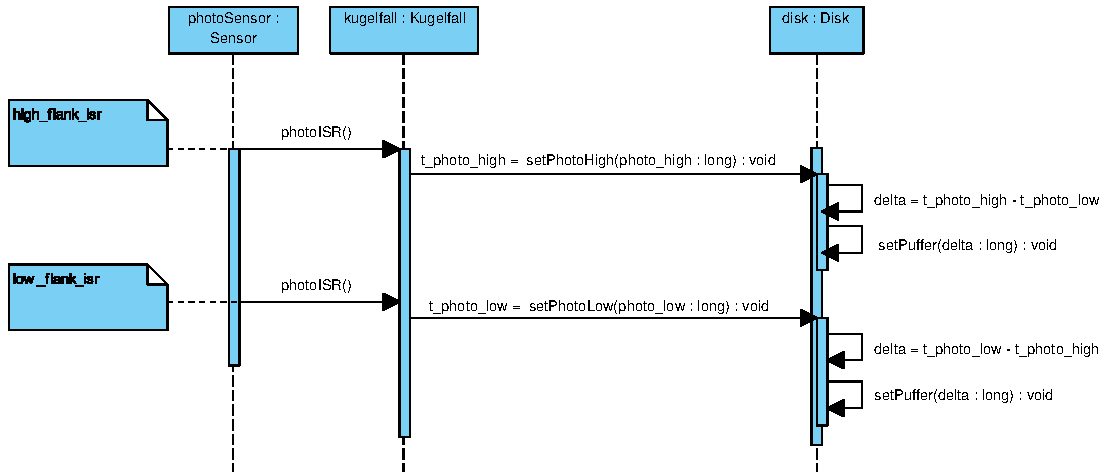
\includegraphics[width=\textwidth]{abb/photoISR_cropped}
	\caption{Ablauf bei der Methode \method{photoISR} von Klasse \class{Controller}}
	\label{fig:photoISR}
\end{figure}
So wird die  Methode \method{photoISR()} in Folge von steigenden und fallenden Flanken des Photosensor aufgerufen.
Die Werte mittels der Methode \method{setPhotoHigh()} bzw. \method{setPhotoLow()} gesichert.
Dabei wird zuerst die Differenz der Werte berechnet und diese dann mit der Methode \method{setPuffer()} innerhalb des Ringpuffers gespeichert.
%Zur Unterscheidung der steigenden und fallenden Flanken dient die boolesche Variable \attr{isPhotoHigh}.

%Denn es stehen mit diesem Ringpuffer nicht nur auf der letzte Wert, sondern die letzten 20 Werte zur Verfügung.

Diagramm \ref{fig:hallISR} zeigt den Ablauf zum Festhalten der Messwerte des Hallsensor mittels \method{hallISR()}.
\begin{figure}[htbp]
	\centering
	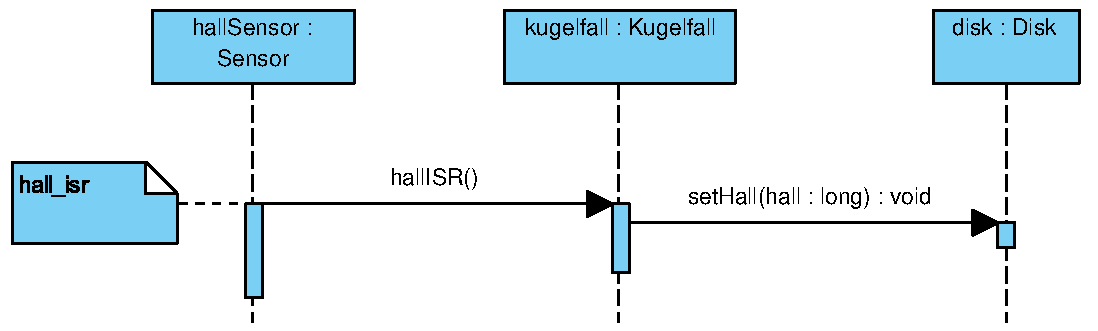
\includegraphics[width=0.8\textwidth]{abb/hallISR_cropped}
	\caption{Ablauf bei der Methode \method{hallISR} von Klasse \class{Controller}}
	\label{fig:hallISR}
\end{figure}
So wird die Methode \method{hallISR()} in Folge einer steigenden Flanke aufgerufen und die Werte Mittels der Method \method{setHall()} gespeichert.
Der aktuelle Wert kann mittels \method{getHall()} ausgelesen werden.